\section{Chapter 7: Space Perception}
\graphicspath{ {pngs/ch7/} }

\secttoc

Interactive 3D computer graphics are inexpensive, but uneducated designs are
ineffective. We are used to the three dimensional, but it does not add much
information compared to a 2D display. Motion parallax may be the strongest cue
we have, but only in limited situations.

\begin{mdframed}
\subsection{Depth Cue Theory}
\begin{multicols}{2}
\begin{compactdesc}
\item[List of monocular depth cues]:
    \begin{compactenum}
    \item linear perspective
    \item texture gradient
    \item size gradient
    \item occlusion
    \item depth of focus
    \item shape-from-shading
    \item vertical position
    \item relative size to familiar objects
    \item cast shadows
    \item depth-from-eye accomodation (non-pictorial)
    \item structure-from-motion (kinetic depth, motion parallax) (needs moving picture )
    \end{compactenum}
\item[List of binocular depth cues]:
    \begin{compactenum}
    \item eye convergence
    \item stereoscopic depth
    \end{compactenum}
\item[Perspective cues] :
    \begin{compactenum}
    \item parallel lines converge to a point
    \item objects at a distance appear smaller than nearby ones
    \item uniformly textured surfaces, where the texture elements become
        smaller with distance
    \end{compactenum}

\end{compactdesc}
\end{multicols}
\end{mdframed}
\begin{mdframed}
\begin{multicols}{2}
\begin{compactdesc}

\item[Size constancy] we perceive the actual size of an object instead of its
    size on the picture. Depth cues can mislead us into finding a difference
    in size in two same-size elements.
\item[Wrong viewpoint?] significant distortions can occur. People can adapt
    after a few minutes. Can persist during extreme conditions and motion,
    so it is best if projection parallel
\item[Occlusion] Object is either behind or in front of another. Best depth
    cue, but provides only binary information.
\item[Shading models] used in shape-by-shading. Key choice: not realism, but
    how well is surface shape revealed?
    \begin{compactenum}
    \item Lambertian -- computationally easy
    \item Specular -- glossy
    \item Ambient -- light from surroundings
    \item Cast shadows
    \end{compactenum}
\item[Light is assumed] to come from above.
\item[Cushion maps] treemap with poofy leaf shading, easier to see
    hierarchy.
\item[Surface texture] can provide information about shape.
\item[Draped grid,] a simple texture, can help reveal surface shape
\item[Cast shadows] form strong depth cues, especially during motion. Fuzzy
    edges are best, better in uncluttered scenes.
\item[Distance and familiarity] objects of known size, arranged meaningfully.
\item[Depth of focus] blur is an ambiguous depth cue. Can be properly computed
    if eye position is known
\item[Eye Accomodation] (amount of focus) isn't used as a depth cue
\item[Structure-from-Motion] rotation, parallax background, oscillatory
    motion about the vertical axis
\item[Eye convergence] non-optimized geometric calculation, only good at arm's
    length.
\item[Diplopia] double-vision.
\item[Stereoscopic depth] small disparities detected in images from two eyes.
    Diplopia can limit.
\end{compactdesc}

\end{multicols}\end{mdframed}


\begin{mdframed}
\begin{multicols}{2}
\begin{compactdesc}
\item[Problems with Stereoscopic displays] People don't like on-screen. In the
    real world, double images of nonattended peripheral objects can be ignored.
    In computers, the lack of depth of focus makes this difficult.
\item[Frame cancellation] object is seen in only one eye, or partially so.
    Acts as an occlusion depth cue, the object seems behind the
    window, breaks the effect.
\item[The Vergence-Focus Problem] (con)vergence of eyes depends on focus
    The disparity between the focus on the screen and the constant vergence can
    cause eyestrain.
    Problem declines with age.
\item[Effective stereoscopic displays]
    Use highest resolution. Screen disparity should be less than 0.03 times the
    distance to the screen.
    Can't make absolute depth judgements.
    Most useful if objects are at 30m or less.
\item[Cyclopean scale] to manage diploplia problems.
    Scale the scene around a center point between the
    right and left viewpoints; the nearest part of the
    scene comes to a point just behind the screen.
\item[Virtual eye separation]
    Equations. If VES is smaller than the actual, depth is decreased. However,
    the brain is imperfect and weighs depth cues differently.
\item[Artificial spatial cues] Dropping lines from a floating object to a
    ground plane.
    Features are artificially added, but it's a natural depth cue.
\item[Halo] around occluding edges of foreground objects. Improves edge contrast,
    which improves occlusion detection. Good for streamlines.
\item[Proximity luminance covariance] ``fog.'' Contrast with background is
    reduced with distance.
    \emph{Atmospheric depth}.
\end{compactdesc}
\end{multicols}\end{mdframed}


\begin{mdframed}
\begin{multicols}{2}
    \begin{figure}[H]
        \centering
        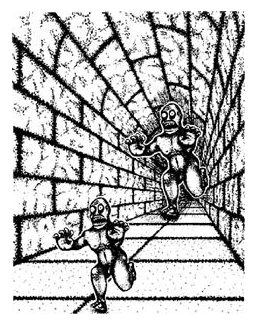
\includegraphics[width=0.6\linewidth]{perspective_illusion.png}
        \caption{Strong perspective cues distort the size of the figures,
        though they are the same.}
    \end{figure}
    \begin{figure}[H]
        \centering
        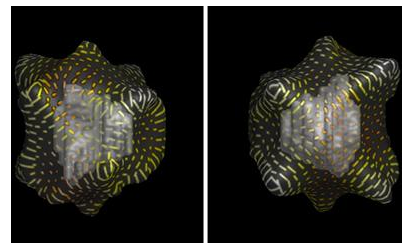
\includegraphics[width=\linewidth]{transparent_textures.png}
        \caption{Designed to reveal surface shape so that another surface can
        be seen beneath.}
    \end{figure}
\end{multicols}
\begin{multicols}{3}
    \begin{figure}[H]
        \centering
        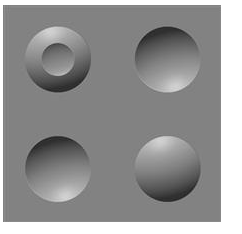
\includegraphics[width=0.15\textwidth]{assume_from_above.png}
        \caption{Brain assumes light comes from above}
    \end{figure}

    \begin{figure}[H]
        \centering
        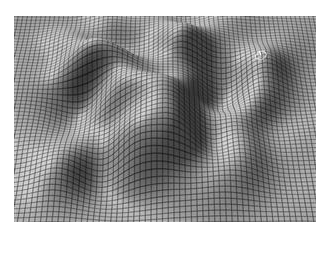
\includegraphics[width=0.2\textwidth]{draped_grid.png}
        \caption{Draped grids can reveal surface shape.}
    \end{figure}
    \begin{figure}[H]
        \centering
        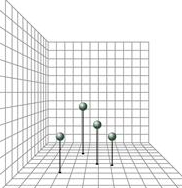
\includegraphics[width=0.2\textwidth]{droplines.png}
        \caption{Dropping lines to a ground plane is an effective artifical
        spatial cue.}
    \end{figure}

\end{multicols}
\end{mdframed}


\begin{mdframed}
\subsection{Combination and Tasks}
\begin{multicols}{2}
\begin{compactdesc}
\item[depth cues in combination] people give depth cues different weight,
    it is not enough to use one type of cue. Combination rules of cues is not
    a unified theory. Could be ad-hoc, depending on scene
\item[task-based space perception] the rest of this chapter is about:
    \begin{compactenum}
    \item tracing 3D paths in graphs
    \item judging morphology of surfaces
    \item finding patterns of points in 3D
    \item finding shapes of 3D paths
    \item judging relative positions of objects
    \item judging relative movements of self
    \item reaching for objects
    \item judging ``up'' direction
    \item feeling a sense of presence
    \end{compactenum}
\end{compactdesc}
\end{multicols}\end{mdframed}



\begin{mdframed}
\subsection{Tracing data paths}
\begin{multicols}{2}
\begin{compactdesc}
\item[Will 3D structures] reveal more data than 2D ones?
\item[Cone trees] can display many more nodes than 2D layouts, but the user
    must navigate to see them
\item[Hyperbolic trees (2D)] hide nodes on an exponential scale, it is easier to
    navigate the tree rapidly.
\item[Path crossings] are the greatest source of errors in reading graphs,
    trees can always be laid out without crossings. Not always the case for
    node-link structures.
\item[Stereo, head-coupled] perspective helped reduce errors with many graph
    nodes, better than 2D.
\item[Occlusion and halos] applied to links can help.
\end{compactdesc}

    \begin{figure}[H]
        \centering
        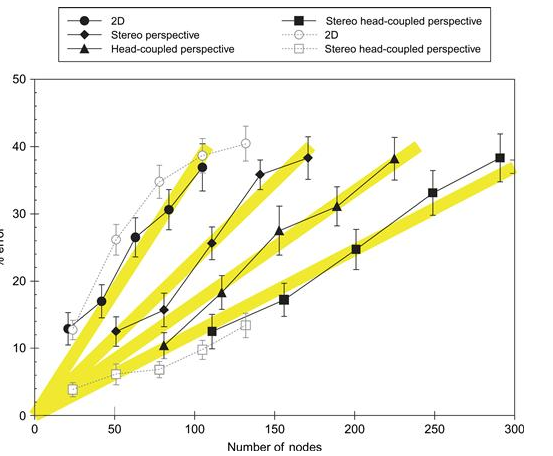
\includegraphics[width=0.4\textwidth]{node_vis_experiment.png}
        \caption{Increase in errors when number of nodes increases.}
    \end{figure}
\end{multicols}\end{mdframed}



\begin{mdframed}
\begin{multicols}{2}
    \begin{figure}[H]
        \centering
        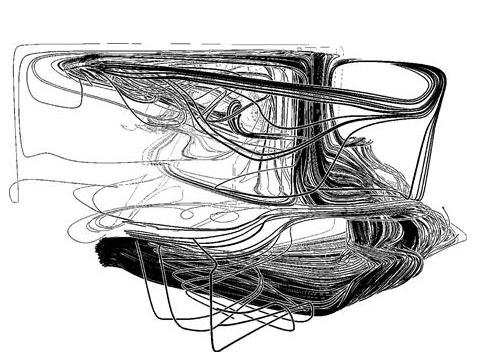
\includegraphics[width=0.4\textwidth]{streamlines.png}
        \caption{Halos enhance occlusion when objects have the same color or
        minimal luminance differences.}
    \end{figure}
    \begin{figure}[H]
        \centering
        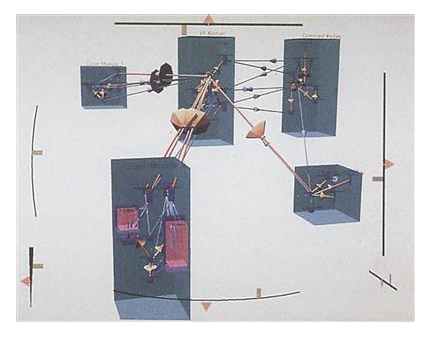
\includegraphics[width=0.4\textwidth]{3d_graph.png}
        \caption{Object-oriented software as a 3D graph}
    \end{figure}

\end{multicols}\end{mdframed}



\begin{mdframed}
\subsection{Judging morphology of surfaces}
\begin{multicols}{2}
\begin{compactdesc}
\item[Simulating real-world] surfaces can help tremendously by leveraging
    Gibson's affordance theory
\item[Hard to predict] who reacts better to different kinds of shading
    techniques. The best seems to involve stereo and/or motion in combination
    with any shading (Lambertian or specular).
\item[Conformal textures] the same texture contained in different boundaries
    can give different effects.
\item[Contours] can give precise height and supplementary shape/gradient
    information.
\item[Guidelines] A simple lighting model can be more effective, as it models
    the brain's model more closely than a photorealistic rendering. Motion
    can decrease time for user to adjust to stereoscopic display.
\item[Bivariate maps] Obvious: shape and surface color. Color cannot change
    rapidly, so it is best to use luminance if the variable changes fast.
\end{compactdesc}
    \begin{figure}[H]
        \centering
        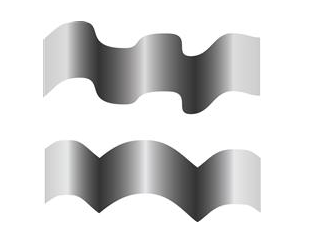
\includegraphics[width=0.4\linewidth]{same_texture_diff_shape.png}
        \caption{Left to right, these gray values are the same, the contours
        are the same.}
    \end{figure}

\end{multicols}\end{mdframed}




\begin{mdframed}
\subsection{Patterns of points in space and in 3D trajectories}
\begin{multicols}{2}
\begin{compactdesc}
\item[Stereoscopic and structure-from-motion] are the most effective cues for
    3D scatterplots.
\item[Easier to perceive cloud] can be formed by treating each point as a flat
    surface and orienting it using statistical methods. This reveals global
    shape and shows individual points as well.

\item[Line rendering for a 3D trajectory] with motion-parallax or stereoscopic viewing, and
    occasional drop lines to the ground.
\item[Tube/box trajectory] gives perspective and shape-from-shading cues,
    especially if rings are drawn around the path
\item[Box trajectory] may also convey roll information.
\end{compactdesc}
    \begin{figure}[H]
        \centering
        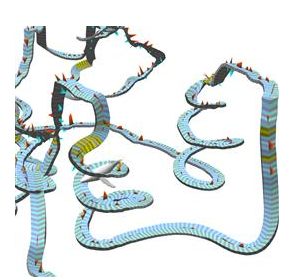
\includegraphics[width=0.5\linewidth]{whale_trajectory.png}
        \caption{Trajectory of a humpback whale bubble-net feeding shown using
        an extruded box.}
    \end{figure}

\end{multicols}\end{mdframed}



\begin{mdframed}
\subsection{Judging relative positions of objects in space, including the Self}
\begin{multicols}{2}
\begin{compactdesc}
\item[Stereoscopic depth] plays a minimal role beyond 30m.
\item[Diverse] 3D environments make it difficult to make generalized
    guidelines. It is best to consider all of the depth cues when finding
    relative positions is important
\item[Self-movement] can be simulated using several visual parameters, called
    \emph{vection}.
    \begin{compactdesc}
    \item[Field size] larger screen, stronger vection
    \item[Foreground/background] stronger if background is perceived as more
        distant
    \item[Frame] stronger if there is a static foreground between the
        observer and the moving background
    \item[Stereo] can help determine if background/foreground is moving,
        stronger effect.
    \end{compactdesc}
\item[Simulator sickness] caused by conflicting cues between vision and the
    inner ear.
\end{compactdesc}

\end{multicols}\end{mdframed}




\begin{mdframed}
\subsection{Selecting and positioning in 3D}
\begin{multicols}{2}
\begin{compactdesc}
\item[Reaching for and manipulating objects] can be important. It is best
    to provide a proxy for the user's hand in the simulation.
\item[Effective Depth cues] stereoscopic display and motion parallax
    coupled with head position. The latter seems more important.
\item[Translational offsets] are easily adapted to
\item[Rotational offsets] are not. Takes weeks to adapt, may not even be
    complete.
\item[Contact with objects] is also important, but difficult to simulate
\end{compactdesc}
\end{multicols}\end{mdframed}




\begin{mdframed}
\subsection{Judging the Up direction and Presence in 3D}
\begin{multicols}{2}
\begin{compactdesc}
\item[This is mainly space research] to help people orient themselves in
    a gravity-free environment
\item[Linear grid] on the virtual floor and walls helps
\item[Familiar objects] also help
\item[Presence] vividly three dimensional. Achieved with a high frame rate and
    a high level of detail
\item[Stereoscopic display] does not help with presence.
    Provides little extra information.
\end{compactdesc}
\end{multicols}\end{mdframed}


